\documentclass[11pt]{article} 
% ~~~~~~~~~~~~~~~~~~~~~~~~~~~~~~~~~~~~~~~~~~~~~~~~~~~~~ %
\input{./Scripts/packages}	
\input{./Scripts/ridefinitions}
\input{./Scripts/figuresgraphicalsettings}
\input{./Scripts/tablesgraphicalsettings}
\input{./Scripts/newcommands}
% Definition of blocks:
\tikzset{%
  block/.style    = {draw, thick, rectangle, minimum height = 3em,
    minimum width = 3em},
  sum/.style      = {draw, circle, node distance = 2cm}, % Adder
  input/.style    = {coordinate}, % Input
  output/.style   = {coordinate} % Output
}
% Defining string as labels of certain blocks.
\newcommand{\suma}{\Large$+$}
\newcommand{\inte}{$\displaystyle \int$}
\newcommand{\derv}{\huge$\frac{d}{dt}$}
% ~~~~~~~~~~~~~~~~~~~~~~~~~~~~~~~~~~~~~~~~~~~~~~~~~~~~~ %

\title{\Huge ELEC-E8101 Group project: \\ Lab B report \\ Group 11}
\date{\today}
\author{HOUILLE Florent, MONTE SASTRE Enrique, SOULARD Yoann, WANG Tong}


\begin{document}
\maketitle

%/////////////////////////////////////////////////////////////%
%/////////////////////////TASK 5.1/////////////////////////%
%/////////////////////////////////////////////////////////////%
\subsection*{Reporting of Task 5.1}

We implemented our PID with the values we obtained in lab A. Unfortunately, the sampling time (42ms) was not working at all. The robot's wheels were just stuck, making a nearly imperciptible back and forth movement. If the sampling time would have been too high, the system would have been unstable and the command would have maxed the limit out right at the beginning. So we didn't find a good reason to explain this behaviour. We tried to bend the robot to force the wheels in one particular direction, but still they are alterning quickly between forward and backward movement.
So instead we used the minimum sampling time (5 ms) and tuned the PID's parameter to finally obtain :

\begin{equation*}
K_p=-250   ;   K_i=-500   ;   K_d=-0.6
\end{equation*}

Actually these parameters were difficult to tune because the robot's behaviour is highly depend of its initial angle. For instance sometimes it could stay up for more than 5 seconds and other times it fell in only 1 second with the exact same parameters set. We decreased $K_p$ to get a smoother behaviour around the null angle (i.e. improve stability, prevent jitters). We decreased integral term to prevent overshoot (once the robot reached the null angle, it was falling the other side). We increased derivative term so that the robot is better ``aware'' that it is going to fall down and can act before it's too late. Here is a result we recorded with Simulink :

\begin{figure}[H]
\centering
\subfloat[$u(t)$]{
  	\includegraphics[width=\linewidth/2]{LabB/Task51_u.pdf}
  }
  \\
  \subfloat[$\theta_b(t)$]{
  	\includegraphics[width=\linewidth/2]{LabB/Task51_thetab.pdf}
  }
   \subfloat[$x_w(t)$]{
  	\includegraphics[width=\linewidth/2]{LabB/Task51_xw.pdf}
  }
  \caption{Simulation results (the robot falls after 5.5 seconds)}
  \label{fig:fig1}
\end{figure}

The command goes at its maximum value at $t=5 s$. It corresponds to the time when the robot stops moving (i.e. $x_w$ is stabilized), before going the other way. We think this brutal command is the reason why the robot fell down.
One can also notice that the command is oscillating. This might be due to high frequency noises coming from the sensors and then transmitted to the PID's derivative action (we didn't use any filter).

%/////////////////////////////////////////////////////////////%
%/////////////////////////TASK 5.2/////////////////////////%
%/////////////////////////////////////////////////////////////%
\subsection*{Reporting of Task 5.2}

%/////5.2.1/////%
5.2.1 Here are the controllability $\mathcal{C}$ and observability $\mathcal{O}$ matrices in parametric and numeric form (according to lab A state-space):

\begin{equation*}
\mathcal{C}=
	\begin{bmatrix}
	B & AB & AAB
	\end{bmatrix}
	=1.10^5
	\begin{bmatrix}
	0 & 0 & 4.10^{-4} & \approx0 \\
	4.10^{-4} & \approx0 & -0.3087 & -1.44.10^{-2} \\
	0 & 0 & -1.6.10^{-3} & \approx0 \\
	-1.6.10^{-3} & \approx0 & 1.3216 & 6.15.10^{-2}
	\end{bmatrix}
\end{equation*}
\begin{equation*}
\mathcal{O}=
	\begin{bmatrix}
	C \\
	AC \\
	AAC \\
	AAAC \\
	\end{bmatrix}
	=1.10^6
	\begin{bmatrix}
	0 & 0 & \approx0 & 0 \\
	0 & 0 & 0 & \approx0 \\
	0 & 3.3.10^{-3} & 1.10^{-4} & -1.10^{-4} \\
	0 & -2.7943 & -0.0262 & 0.0587
	\end{bmatrix}
\end{equation*}
\begin{equation*}
\Delta\mathcal{C}=-1.10^{-5} \;\; \Delta\mathcal{O}=0
\end{equation*}

$\mathcal{C}$ matrice is full-rank (4), therefore the system is controllable. 
$\mathcal{O}$ matrice is not full-rank, therefore the system is non-observable.



\end{document}

%	INLINE EQUATION FORMAT
% This is an example sentence with this formula : $x=50$

%	BOLD TEXT
%\textbf{Type text here}

%	FRACTION
%\frac{Numerator}{Denominator}

%	 MATRIX with brackets like this : [ ]
%\begin{equation*}
%x=
%	\begin{bmatrix}
%	x_11 & x_12\\
%	x_21 & x_22\\
%	x_31 & x_32\\
%	\end{bmatrix}
%\end{equation*}

%	SYSTEM OF EQUATIONS
%\begin{align*}
%\begin{cases}
% equation1 left part = equation1 right part\\
% equation2 left part = equation2 right part\\
%\end{cases}
%\end{align*}

%	1 FIGURE centered just after the text, with a description and a number
%\begin{figure}[H]
%  \includegraphics[width=\linewidth]{LabFolder/ImageName.png}
%  \caption{Description of figure}
%  \label{fig:fig1}
%\end{figure}

%	4 FIGURES displayed 2 by 2 , with a global description
%\begin{figure}[H]
%  \includegraphics[width=\linewidth/2]{LabA/Task45_xw.pdf}
%  \includegraphics[width=\linewidth/2]{LabA/Task45_Thetaw.pdf}
%  \includegraphics[width=\linewidth/2]{LabA/Task45_vw.pdf}
%  \includegraphics[width=\linewidth/2]{LabA/Task45_d.pdf}
%  \caption{Simulation results}
%  \label{fig:fig4}
%\end{figure}

%	4 FIGURES displayed 2 by 2 , with a description for each
%\begin{figure}[H]
%\begin{subfigure}[b]{0.5\linewidth}
%  \includegraphics[width=\linewidth]{LabA/Task48_vmDiscXTraMass0kg500g.pdf}
%  \caption{description 1}
%\end{subfigure}
%\begin{subfigure}[b]{0.5\linewidth}
%  \includegraphics[width=\linewidth]{LabA/Task48_vmDiscXTraMass1kg.pdf}
%    \caption{description 2}
%\end{subfigure}
%\begin{subfigure}[b]{0.5\linewidth}
%  \includegraphics[width=\linewidth]{LabA/Task48_vmDiscXTraMass3kg.pdf}
%    \caption{description 3}
%\end{subfigure}
%\begin{subfigure}[b]{0.5\linewidth}
%  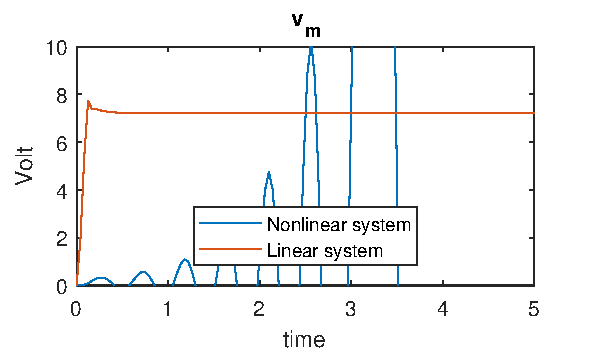
\includegraphics[width=\linewidth]{LabA/Task48_vmDiscXTraMass25kg.pdf}
%    \caption{description 4}
%\end{subfigure}
%  \caption{General description}
%  \label{fig:fig7}
%\end{figure}
